\newpage
\section{Students}
First of all if you have never done it, you have to sign up inserting your name, surname, mail address, fiscal code, the unique code that had been given to you by the university personell and a profile image, otherwise you only need to click on the login button.
After the login you will notice that a black bar has appeared near the top of the screen. it contains the voices \textbf{Exam session}, \textbf{Booking board} and \textbf{Booklet}.

\begin{figure}[H]
	\centering
	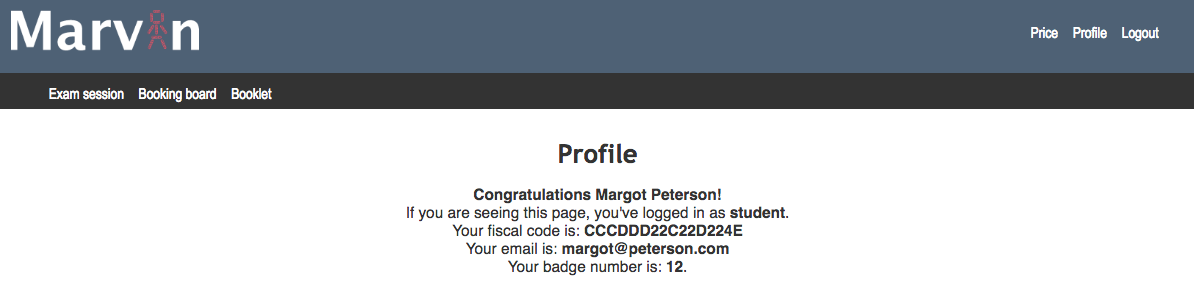
\includegraphics[width=1.0\textwidth]{img/studentProfile.png}
	\caption{Student profile page }
	\label{fig:studentProfile}
\end{figure}

\subsection{Exam Session}
To visualize the list of the exams to which you can subscribe, click on the voice \textbf{Exam session} you will be redirected to a page (similar to the one in Figure~\ref{fig:studentExams}) . If you want to subscribe to an exam, then click on the button \textbf{subscribe} corresponding to that exam.
\begin{figure}[H]
\centering
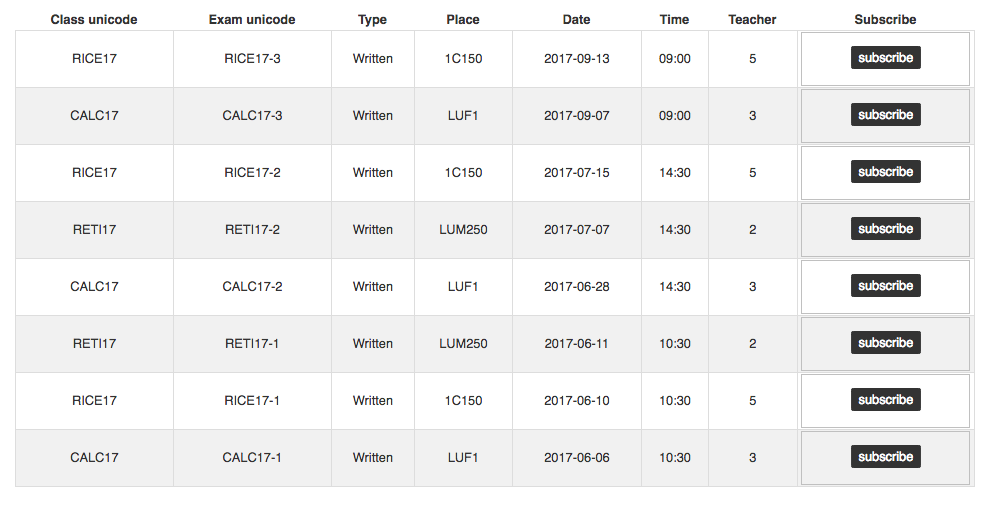
\includegraphics[width=1.0\textwidth]{img/studentExams.png}
\caption{List of exams to which the student can register and to which is already registered.}
\label{fig:studentExams}
\end{figure}
After that you will be redirected to your \emph{booking board}, where you can see all the exams to which you subscribed and also accept the marks of the ones that you passed.

\subsection{Booking board}
If you want to visualize the classes to which you subscribeb, then click on the voice \textbf{Booking board}, you will be redirected to a page (similar to the one in Figure~\ref{fig:studentRecords}).  If a certain exam has a mark, than you can accept it by clicking on the \textbf{confirm} button (if an exam hasn't a mark yet, then the button is unclickable) and you will be redirected to your \emph{booklet} page where you can visualize all the classes thet you passed. When you accept a vote, this one disappears from the booking board and it is saved in the booklet.
\begin{figure}[H]
	\centering
	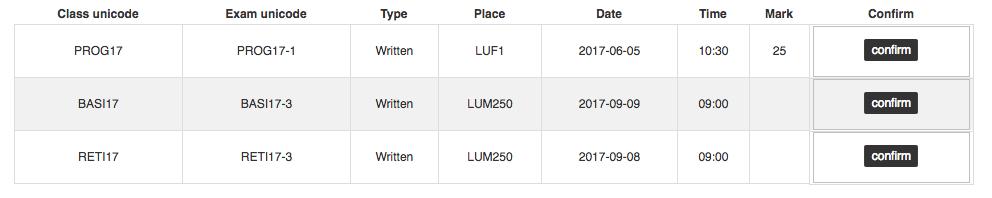
\includegraphics[width=1.0\textwidth]{img/studentRecords.png}
	\caption{List of the exams to which the student is subscribed}
	\label{fig:studentRecords}
\end{figure}

\subsection{Booklet}
To visualize the list of  all the classes that you have passed, click on the voice \textbf{Booklet}, you will be redirected to a page (similar to the one in Figure~\ref{fig:booklet}).
\begin{figure}[H]
	\centering
	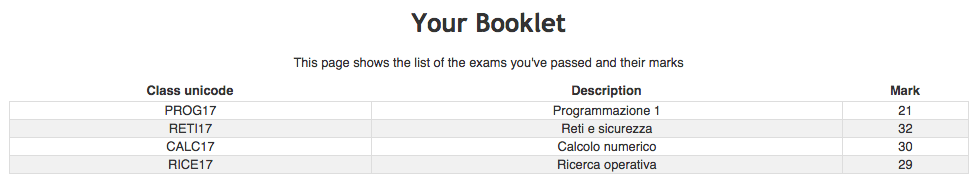
\includegraphics[width=1.0\textwidth]{img/booklet.png}
	\caption{List of the classes passed by the student.}
	\label{fig:booklet}
\end{figure}